\chapter{Appendix}\label{cha:Appendix}

\section{Journal}\label{sec:Journal}
\begin{table}[H]
    \centering
    
\begin{tabular}{||c | c | c || c||} 
 \hline
 Date &  Location & Duration & Activity \\ [0.5ex] 
 \hline\hline
  01.09.2023 & TBZ & 1.5h & Selected and bought \acs{devboard} \\ 
 \hline
 08.09.2023 & TBZ & 2h & Tested \acs{devboard} with demos \\ 
 \hline
  08.09.2023 & TBZ & 0.5h & Noted first ideas for \acs{dmm} \\ 
 \hline
   15.09.2023 & TBZ & 1.5h & Written and signed Project Agreement [\ref{sec:Project Agreement}] \\ 
 \hline
    21.09.2023 & Home & 3h & Created documentation template \\ 
 \hline
    22.09.2023 & TBZ & 2h &  Started writing Journal [\ref{sec:Journal}]\\ 
 \hline
    24.09.2023 & Home & 1.5h &  Made GANTT chart [\ref{sec:GANTT Chart}]\\ 
 \hline
    27.09.2023 & Home & 2h & Written detailed planning and introduction \\ 
 \hline
    29.09.2023 & TBZ & 1.5h & Added mindmap, Lasten-, Pflichtenheft \\ 
 \hline
    06.10.2023 & TBZ & 1h & Started with block diagram (extension PCB) \\ 
 \hline
    20.10.2023 & ETH & 0.5h & Started Altium Project, Schematic template \\ 
 \hline
    23.10.2023 & ETH & 3h & HW Concept / documentation \\ 
 \hline
   23.10.2023 & ETH & 3h & Start schematic / documentation \\ 
 \hline
   25.10.2023 & Home & 2h & Schematic: Current Src, Volt div \\ 
 \hline
   26.10.2023 & ETH & 1.5h & Schematic: Current meas, ERC \\ 
 \hline
   26.10.2023 & Home & 1h & Schematic: Cleanup, Comments, DS Saves \\ 
 \hline
   26.10.2023 & Home & 1h & Documentation \& prepared Interview 1 \\ 
 \hline
  27.10.2023 & TBZ & 1.5h & Documentation: Started with schematic part \\ 
 \hline
  28.10.2023 & Home & 2h & Documentation: schematic parts \\ 
 \hline
  29.10.2023 & Home & 1h & Docu: schematic done, resources cleanup \\ 
 \hline
   29.10.2023 & Home & 0.5h & Layout: Outline, Placement start \\ 
 \hline
   31.10.2023 & Home & 1h & Layout: Placement Done \\ 
 \hline   
   01.11.2023 & Home & 1.5h & Layout: Routing Done \\ 
 \hline
  02.11.2023 & Home & 1h & Layout: Cleanup \& Export \\ 
 \hline
  03.11.2023 & TBZ & - & Interview 1: signed by mala \\ 
 \hline  
  03.11.2023 & TBZ & 1h & Pepared BOM for supplying \\ 
 \hline
  04.11.2023 & Home & 1h & Documentation: PCB, Reflection \\ 
 \hline

\end{tabular}
    \caption{Project Journal 1}\label{tab:Project Journal 1}
\end{table}

\newpage

\begin{table}[H]
  \centering
  
  \begin{tabular}{||c | c | c || c||} 
    \hline
    Date &  Location & Duration & Activity \\ [0.5ex] 
    \hline\hline
    05.11.2023 & Home & 0.5h & STM32 Multicore Debugging \\ 
    \hline
     05.11.2023 & Home & 1h & Documentation: STM32 Multicore Debug \\ 
    \hline
     05.11.2023 & Home & 1h & Boot problems / HW MOD \\ 
    \hline
    09.11.2023 & Home & 3h & Population of 2 Extension PCBs \\ 
    \hline
    11.11.2023 & Home & 0.5h & HW MOD of second DevBoard \\ 
    \hline
    14.11.2023 & Home & 2h & QSPI Write test and documentation \\ 
    \hline
    23.11.2023 & Home & 3.5h & QSPI: tried to Ext. boot \\ 
    \hline
  \end{tabular}
  \caption{Project Journal 2}\label{tab:Project Journal 2}
\end{table}

\newpage



\section{Weekly plans}
\label{sec:Project Planning}

\subsection{KW39 \& 40}
\begin{itemize}
    \item Write introduction
    \item Planning: Cost, Tools, When, Why
    \item Create project diagram (learning process)
    \item ''Lastenheft''
    \item ''Pflichtenheft''
    \item Make a \acs{hw}-Digram for the Extension \acs{pcb}.
    \item Make the schematic of the Extension \acs{pcb}. 
    \begin{itemize}
        \item Part to measure voltage.
        \item Part to measure current.
        \item Part to measure continuity.
        \item Addressable LEDs.
    \end{itemize}
    \item Start with the Layout of the Extension \acs{pcb}.
    \item Reflection of the start of the project.
\end{itemize}




\subsection{KW41 \& 42}
Fall holidays. I planned to invest much time in the holidays, but it turned out that my plans changed, and I was busy.



\subsection{KW43 \& 44}
Mainly catching up.
\begin{itemize}
    \item Make a \acs{hw}-Digram for the Extension \acs{pcb}.
    \item Make the schematic of the Extension \acs{pcb}. 
    \begin{itemize}
        \item Part to measure voltage.
        \item Part to measure current.
        \item Part to measure continuity.
        \item Addressable LEDs.
    \end{itemize}
    \item Make the whole Layout of the Extension \acs{pcb}.
    \item Order the Extension PCB and the components.
    \item Reflection of the start of the project.
\end{itemize}
and maybe if the time is sufficient I could start with implementing the SDRAM and QSPI Flash.



\subsection{KW45 \& 46}
\begin{itemize}
  \item Populate and commission the extension PCB.
  \item Implement QSPI flash with bootloader.
  \item Implement external SDRAM.
  \item Implement touch display. (MIPI DSI, Touch)
\end{itemize}
and maybe if the time is sufficient I could start with learning TouchGFX.

\newpage



\section{GANTT Chart}
\label{sec:GANTT Chart}
\label{fig:GANTT Chart}
\begin{figure}[H]
	\centering
    \framebox{
	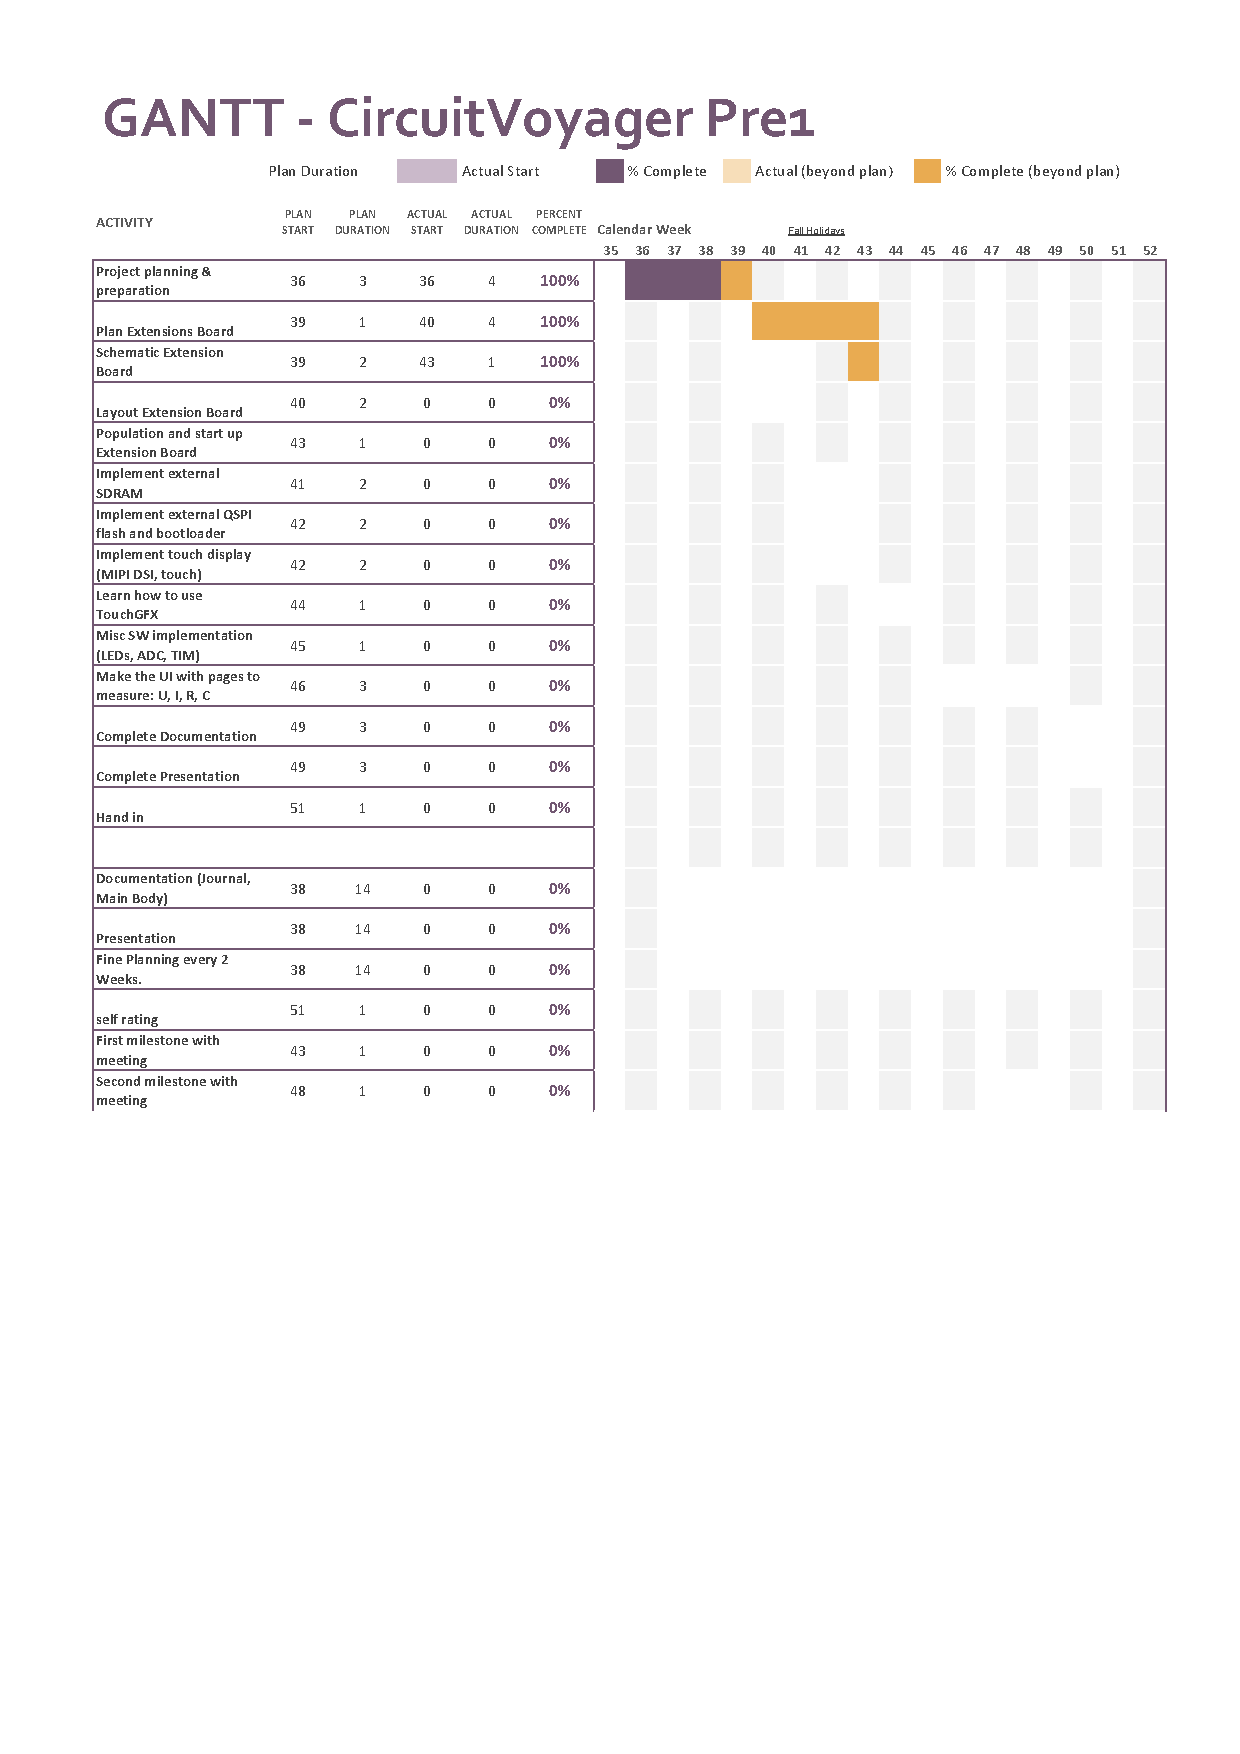
\includegraphics[width=14.5cm]{../../2_Project_Planning/GANTT/GANTT.pdf}}
	\caption{GANTT Chart}
\end{figure}
\newpage




\section{Project Agreement}
\label{sec:Project Agreement}
\begin{figure}[H]
  \label{fig:Project Agreement}
	\centering
    \framebox{
	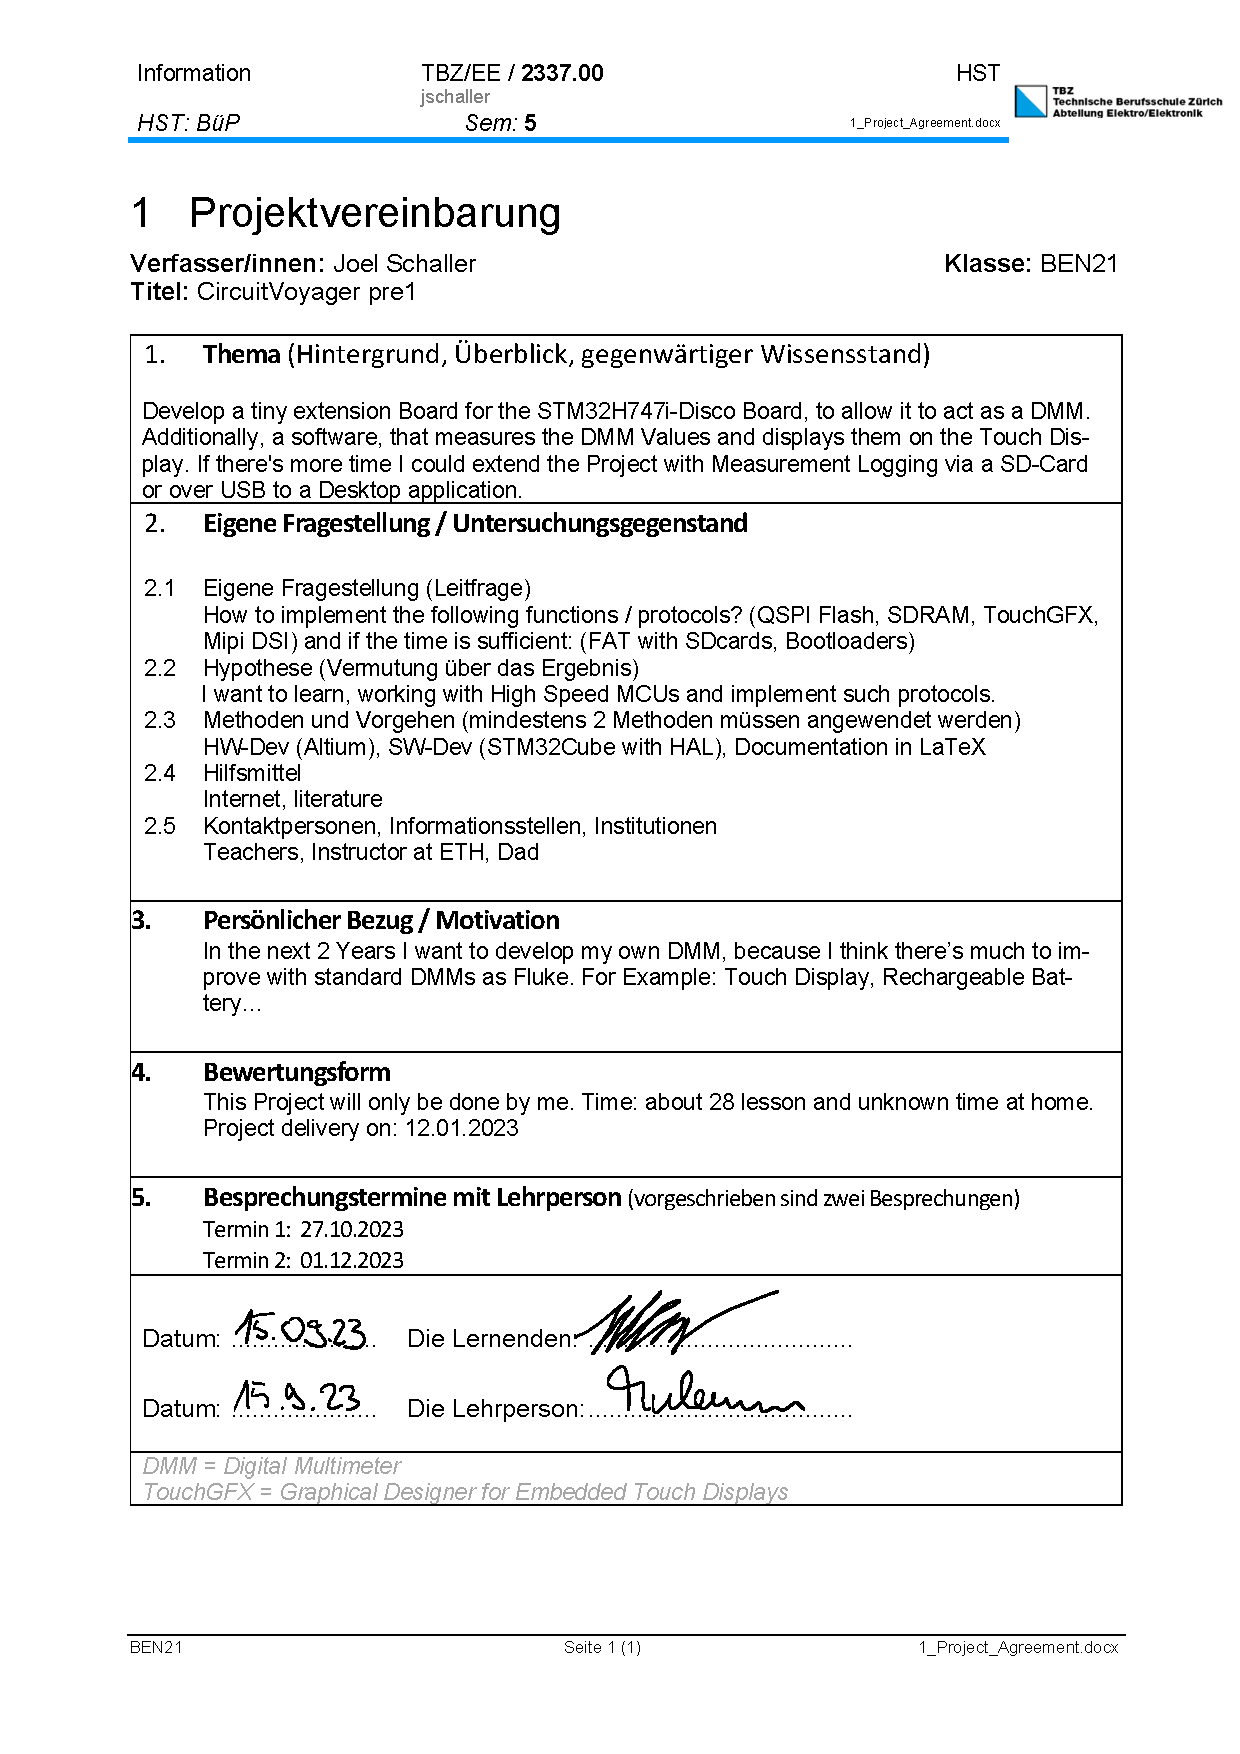
\includegraphics[width=14.5cm]{../../../1_Agreement_Review/1_Project_Agreement_CircuitVoyager_pre1_jschaller_230915.pdf}}
	\caption{Project Agreement}
\end{figure}
\newpage

\section{Interview 1}
\label{sec:Interview 1}
\begin{figure}[H]
  \label{fig:Interview 1}
	\centering
    \framebox{
	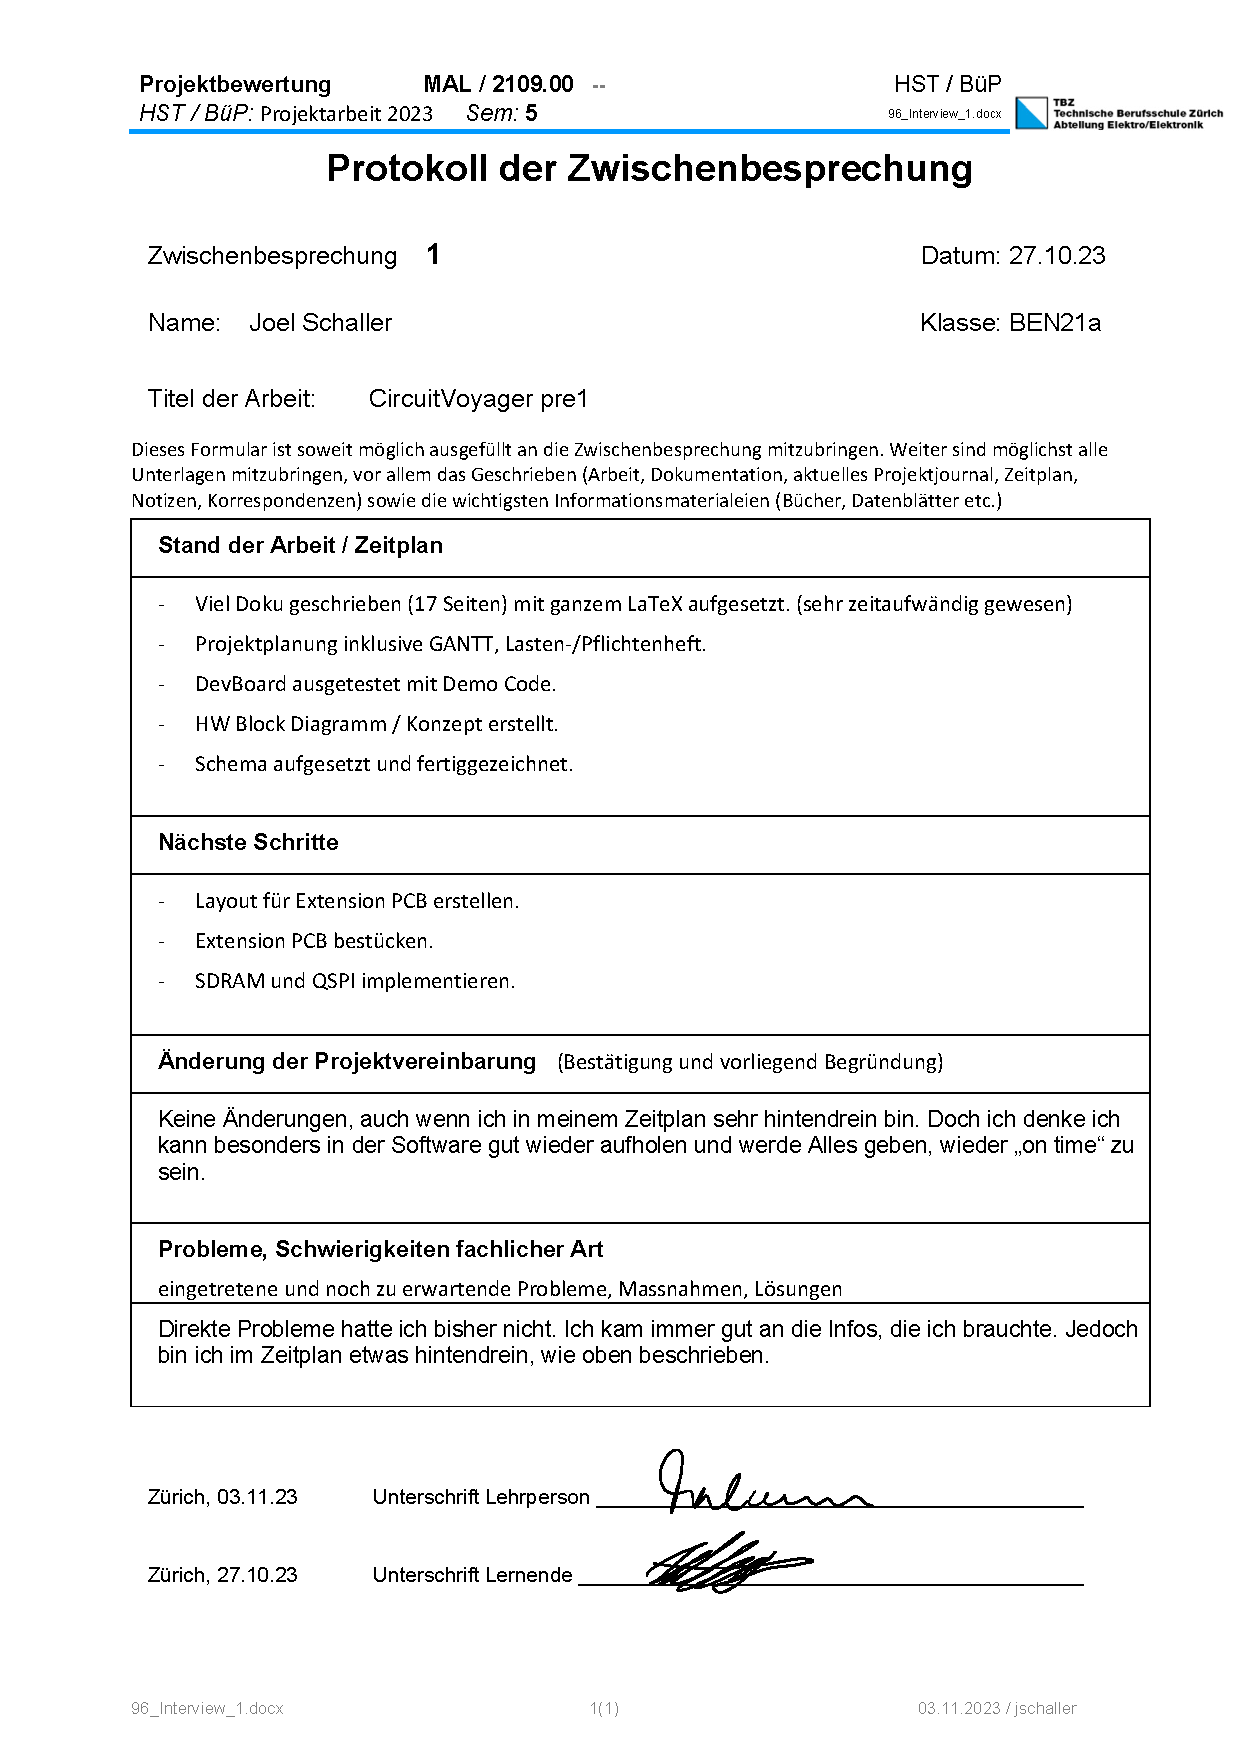
\includegraphics[width=14.5cm]{../../../1_Agreement_Review/96_Interview_1.pdf}}
	\caption{Interview 1}
\end{figure}
\newpage



\section{Extension PCB Schematics}
\label{sec:Extension PCB Schematics}
\begin{figure}[H]
	\centering
	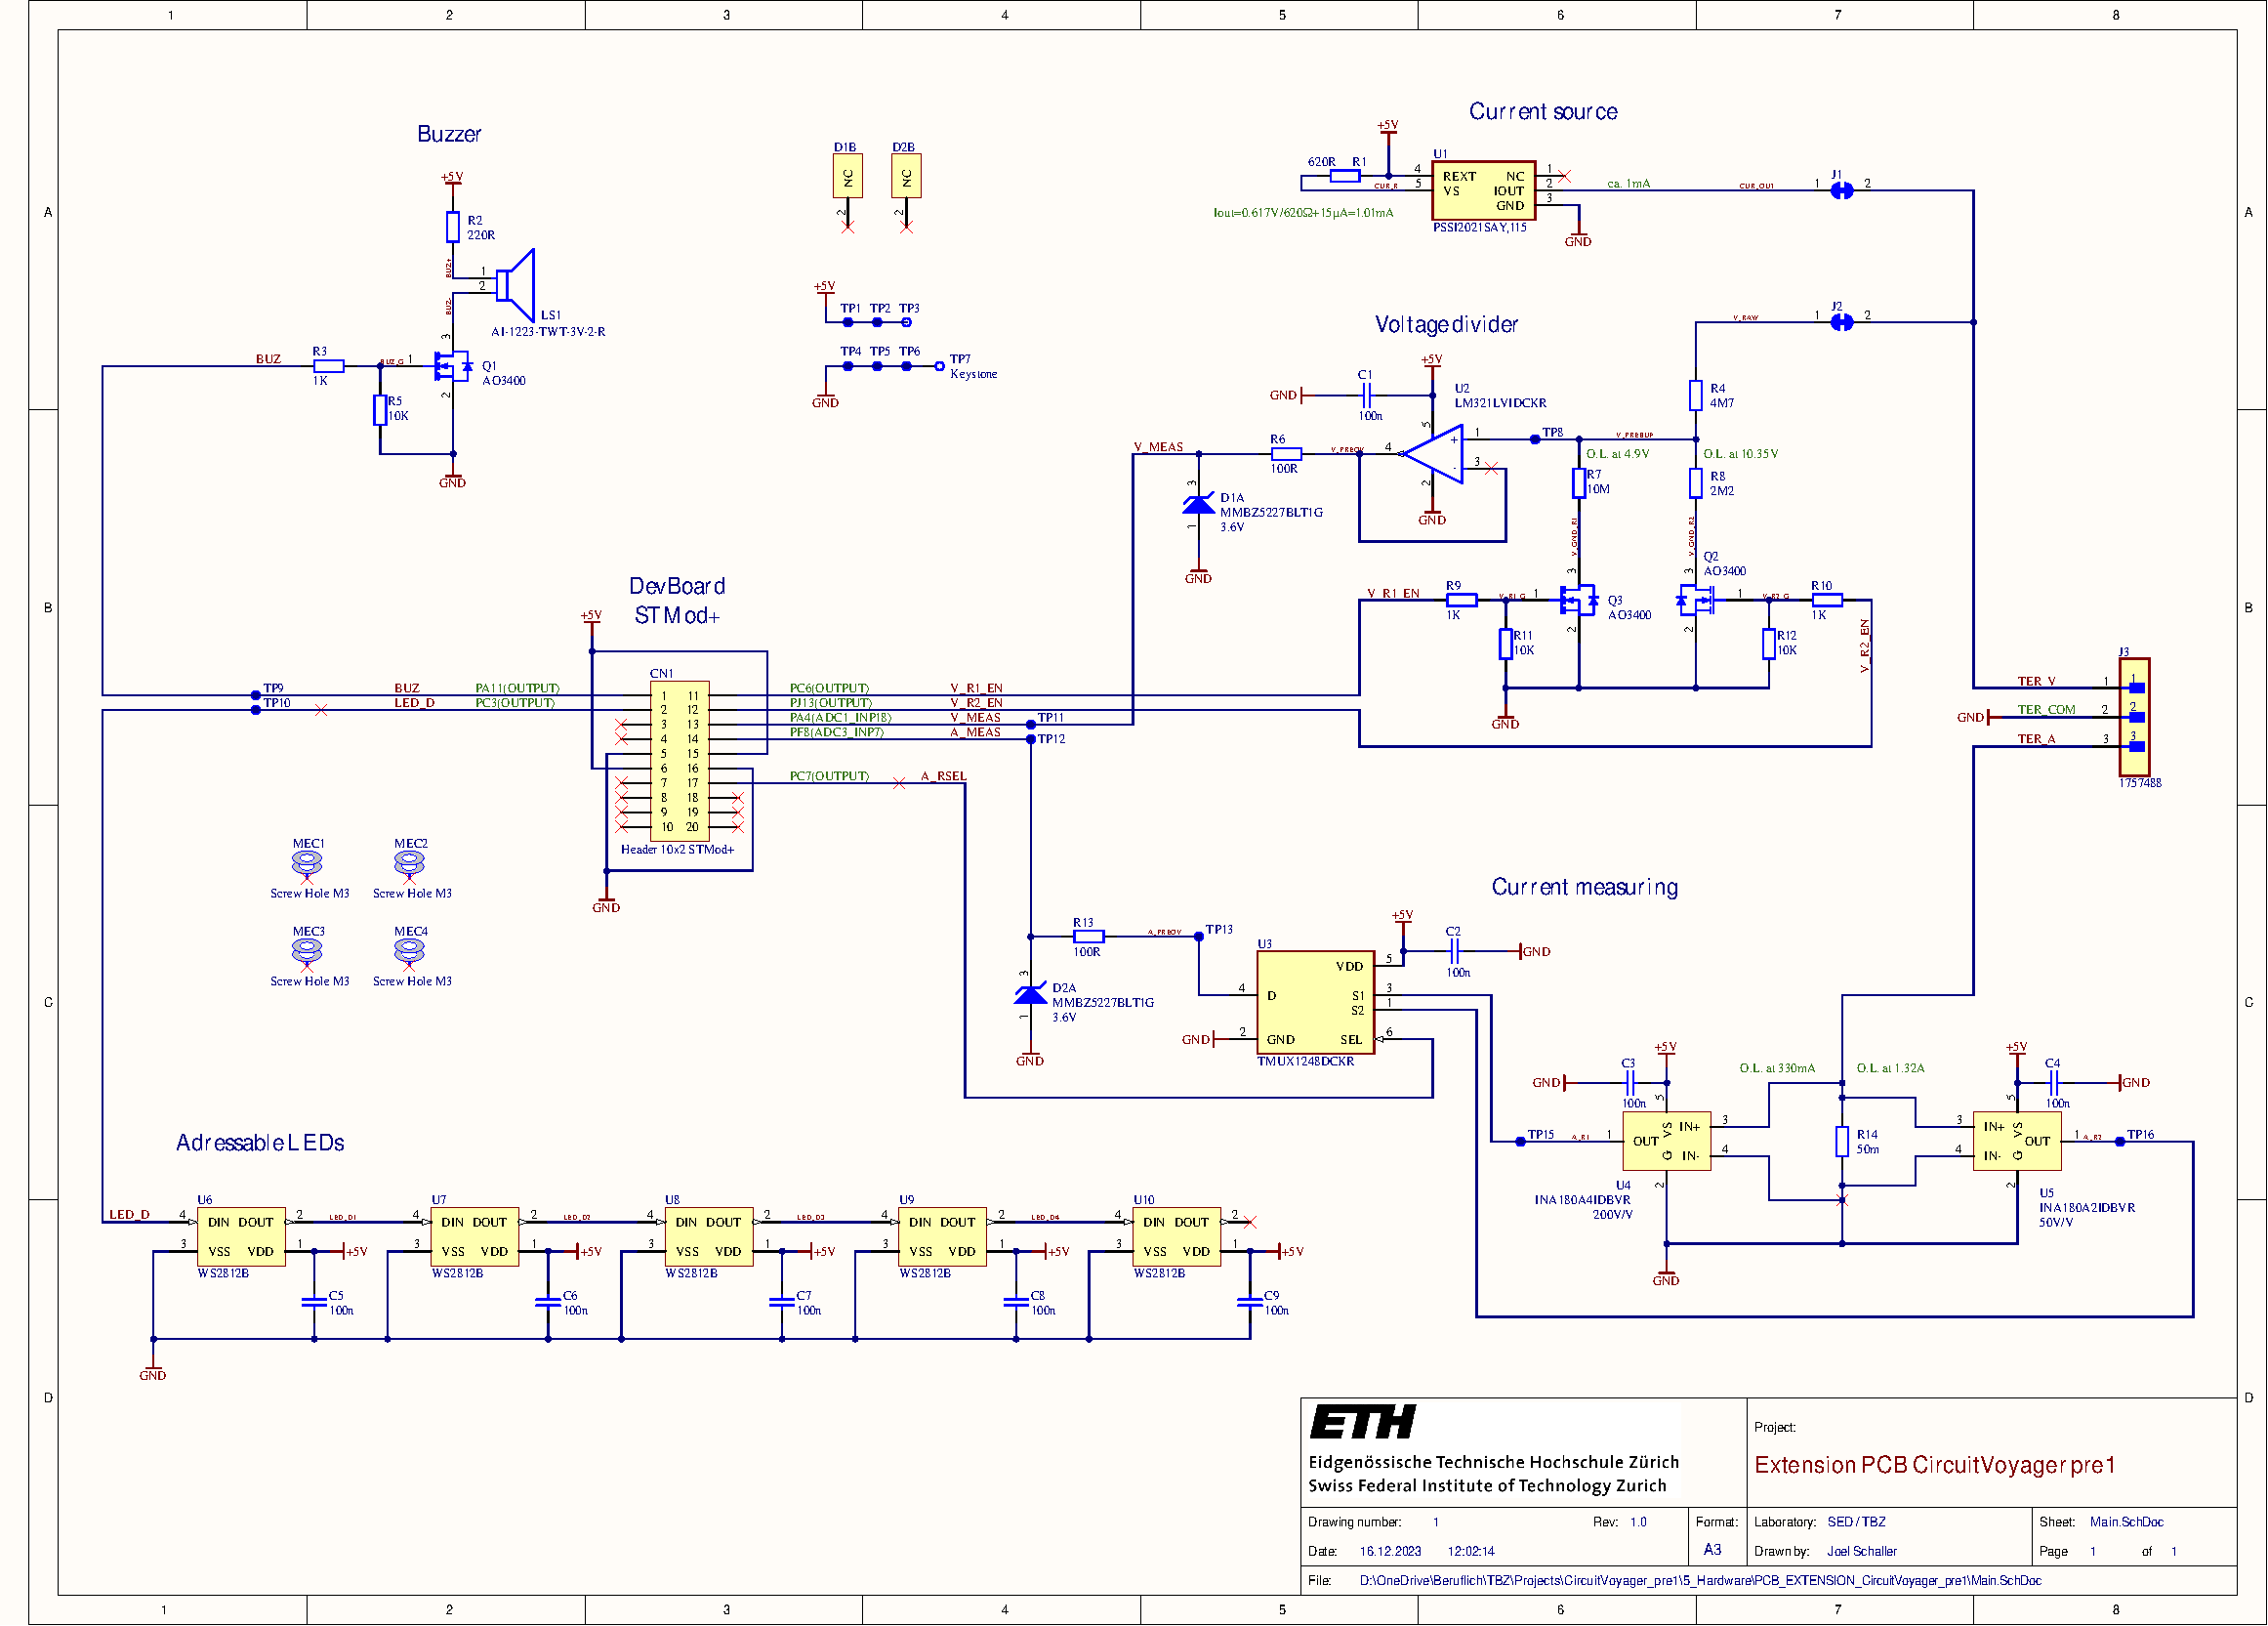
\includegraphics[height=15cm, angle=270]{../../../5_Hardware/PCB_EXTENSION_CircuitVoyager_pre1/Project Outputs for PCB_EXT_CV_PRE1/Schematic_PCB_EXTENSION_CircuitVoyager_pre1.pdf}
	\caption{Extension PCB Schematics}
	\label{fig:Extension PCB Schematics}
\end{figure}


\section{Extension PCB Manufacture 11.23 BOM}
\label{sec:Extension PCB Manufacture 11.23 BOM}
\begin{figure}[H]
	\centering
  \framebox{
	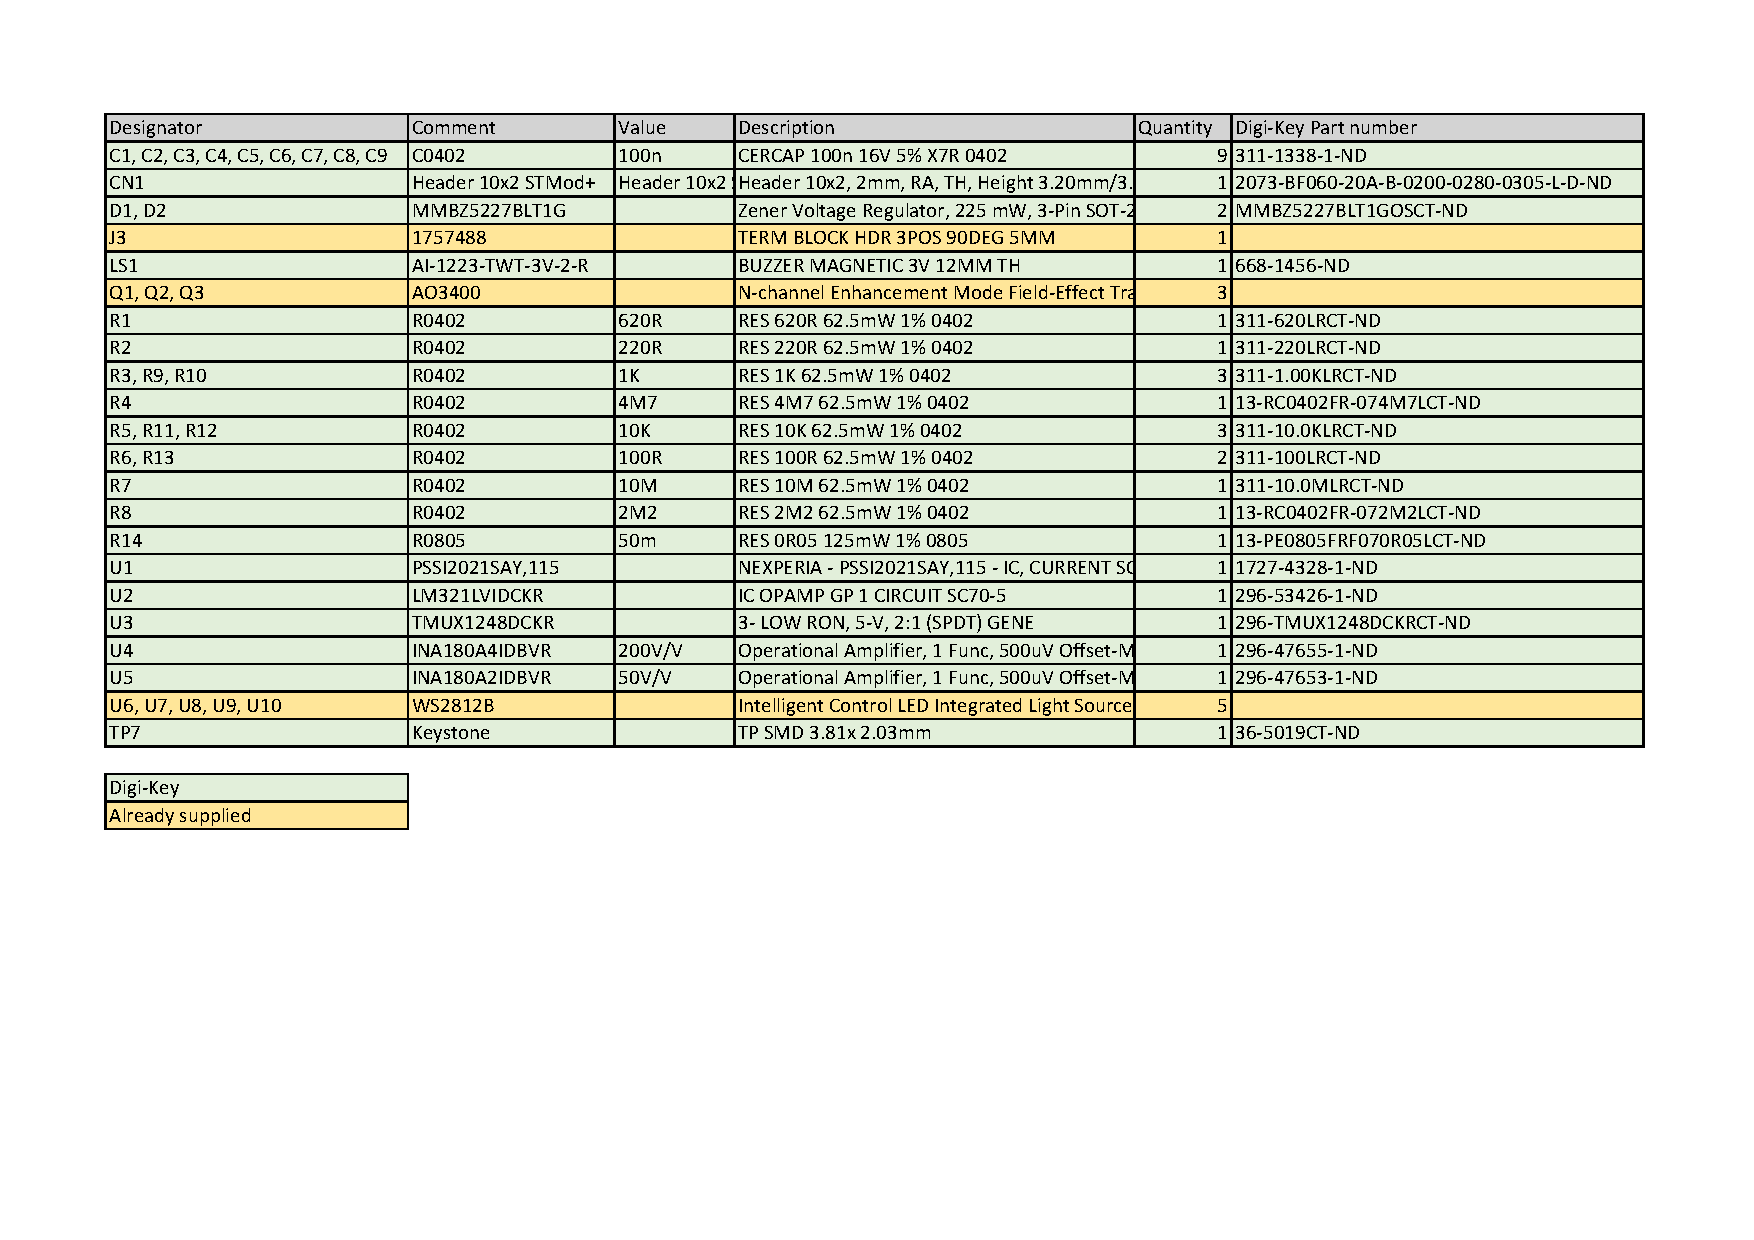
\includegraphics[height=14.5cm, angle=270]{../../../5_Hardware/PCB_EXTENSION_CircuitVoyager_pre1/MANUFACT_2311/BOM-PCB_EXT_CV_PRE1.pdf}
  }
	\caption{Extension PCB Manufacture 11.23 BOM}
	\label{fig:Extension PCB Manufacture 11.23 BOM}
\end{figure}
\newpage